\documentclass[paper=a4, fontsize=11pt, open=any, parskip=half-,
  headings=small, numbers=noenddot, captions=tableheading, toc=flat]{scrreprt}
\usepackage{anchorai}
\usepackage{placeins}
\addbibresource{references.bib}
\graphicspath{{figures/}}

% The short version has no chapters: sections are the top level and run on without page breaks
\renewcommand{\thesection}{\arabic{section}}
\renewcommand{\thefigure}{\arabic{figure}}
\renewcommand{\thetable}{\arabic{table}}
\renewcommand{\theequation}{\arabic{equation}}
\automark[section]{section}
\renewcommand*{\sectionmarkformat}{\textcolor{nusOrange}{\thesection}\hspace{0.6em}}
\setuptoc{toc}{leveldown}
\setcounter{tocdepth}{1}
\setcounter{secnumdepth}{2}
\RedeclareSectionCommand[beforeskip=-1.6\baselineskip, afterskip=0.5\baselineskip]{section}

\begin{document}

\begin{titlepage}
  \global\pagebandfalse
  \begin{tikzpicture}[remember picture, overlay, every node/.style={inner sep=0pt, outer sep=0pt}]
    \coordinate (L) at ([xshift=26mm]current page.north west);
    \coordinate (R) at ([xshift=-26mm]current page.north east);
    \node[anchor=north west] at ([yshift=-20mm]L) {
\includegraphics[height=19mm]{diagrams/nus-logo.pdf}};
    \node[anchor=north east, align=right, font=\sffamily\small, text=nusBlue] at ([yshift=-22mm]R)
      {\textbf{Institute of Systems Science}\\[1.2mm]Intelligent Reasoning Systems\\[1.2mm]\color{muted}Project report};
    \fill[nusBlue] ([yshift=-62mm]current page.north west) rectangle ([yshift=-182mm]current page.north east);
    \fill[nusOrange] ([yshift=-182mm]current page.north west) rectangle ([yshift=-184.5mm]current page.north east);
    \node[anchor=north west, font=\sffamily\bfseries\footnotesize, text=nusOrange] at ([yshift=-80mm]L)
      {\addfontfeature{LetterSpace=12}GROUP PROJECT REPORT\enskip·\enskip SHORT VERSION};
    \node[anchor=north west, font=\sffamily\bfseries, text=white] at ([yshift=-90mm]L)
      {\fontsize{50}{52}\selectfont Anchor\textcolor{nusOrange}{AI}};
    \node[anchor=north west, text width=150mm, font=\sffamily\fontsize{19}{24}\selectfont, text=white] at ([yshift=-113mm]L)
      {Explainable, budget-aware retention planning for gyms};
    \fill[nusOrange] ([yshift=-135mm]L) rectangle ([xshift=24mm, yshift=-136.4mm]L);
    \node[anchor=north west, text width=158mm, font=\sffamily\small, text=white!82!nusBlue, align=left] at ([yshift=-143mm]L)
      {Churn prediction\enskip·\enskip uplift estimation\enskip·\enskip rule-based reasoning\enskip·\enskip case-based reasoning\\[1mm]
       genetic algorithm with an exact CP-SAT benchmark\enskip·\enskip knowledge graph\enskip·\enskip grounded staff assistant};
    \node[anchor=north west, font=\sffamily\bfseries\footnotesize, text=nusOrange] at ([yshift=-200mm]L)
      {\addfontfeature{LetterSpace=12}TEAM};
    \node[anchor=north west, font=\sffamily, text=ink] at ([yshift=-208mm]L) {%
      \renewcommand{\arraystretch}{1.55}%
      \begin{tabular}{@{}p{78mm}l@{}}
        Abdulaziz Ali S Hasanain   & \color{muted}A0350856X \\
        Asiri Mohammed Yahya A     & \color{muted}A0351967N \\
        Binmaneea Khalid Waleed M  & \color{muted}A0355712E \\
      \end{tabular}};
    \draw[rule, line width=0.6pt] ([yshift=-252mm]L) -- ([yshift=-252mm]R);
    \node[anchor=north west, font=\sffamily\small, text=muted] at ([yshift=-256mm]L)
      {National University of Singapore};
    \node[anchor=north east, font=\sffamily\small, text=nusBlue] at ([yshift=-256mm]R)
      {\textbf{Group 16}\enskip·\enskip 25 October 2026};
    \fill[nusBlue] (current page.south west) rectangle ([yshift=5mm]current page.south east);
    \fill[nusOrange] ([yshift=5mm]current page.south west) rectangle ([yshift=6.3mm]current page.south east);
  \end{tikzpicture}
\end{titlepage}
\global\pagebandtrue

\pagenumbering{arabic}
\markboth{Abstract}{Abstract}
\section*{Abstract}

About one gym member in three leaves each year, and most stop attending weeks before they cancel. Retention tools flag members at risk but leave the decision that matters (whom to contact this week, with which offer, within a fixed budget and limited staff hours) to guesswork. AnchorAI makes that decision and explains it. A calibrated ensemble predicts churn on real members; a forward-chaining rule base encodes the gym's playbooks and guardrails; case-based reasoning estimates what each offer would achieve for each member; a genetic algorithm, benchmarked against an exact CP-SAT solver, builds the weekly plan; a knowledge graph adds signals the churn model cannot see; and a grounded assistant answers staff questions from the system's own evidence. Segmentation and churn are evaluated on 4,000 real members of a public dataset; decisions on a documented synthetic scenario layer whose true offer effects are known, which shows that the method works when effects are of this kind, not how large they are in a real gym.

\vspace{0.8\baselineskip}
\noindent
\keyfigure{0.908}{churn F1 on 800 unseen real members (PR-AUC 0.973)}\hfill
\keyfigure{+22--138\%}{more members kept than contacting by risk or by schedule, at equal budget}\hfill
\keyfigure{0.24\%}{largest gap of the genetic algorithm to the proven optimum}\hfill
\keyfigure{96.2\%}{of the assistant's judged sentences supported by its evidence}

\vspace{0.4\baselineskip}
\tableofcontents

\section{Business case, market research and objectives}
\label{sec:intro}

Gym members rarely cancel on impulse: they stop coming first and cancel weeks later, and that lag is the window in which a well-chosen contact can still keep them. The median member retention rate was 66.4\% in 2024 across 175 operators~\cite{hfa2025benchmarking}, and new members are the most fragile: in one fitness centre 63\% stopped before their third month~\cite{sperandei2016adherence}. Current practice produces a list or a score but not a decision. Calendar campaigns spend on members who would have stayed, threshold rules ignore trends, and vendor risk scores give staff a number they cannot interrogate. The proposal's market research found that no vendor publicly exposes constrained allocation, that vendors target risk although targeting by expected response reduces churn more~\cite{ascarza2018futility}, and that the intelligence layer is priced for chains of five or more clubs. AnchorAI is therefore positioned as an \emph{explainable, budget-aware retention planner for operators with one to five clubs}. No real operator was involved: the interviews that shaped the rules were simulated, and every comparison is against baseline policies in our own experiments.

\subsection{Pricing and business value}
\label{sec:pricing}
% Pricing and business value, shared by both reports; each report writes its own heading before \input.
AnchorAI is sold as an annual subscription that bolts onto the operator's existing membership system: US\$199 a month for the first club and US\$149 for each further club up to five, so a three-club operator, the size of our scenario, pays US\$497 a month. It runs on the operator's own machine, language model included: in E8 a local seven-billion-parameter model was as faithful to its evidence as the hosted one (95.1\% of judged sentences supported for each), so there is no fee per question. A hosted and maintained option would cost more, to cover hosting and support; we have not costed it.

The price sits where the gap in the market is (\cref{tab:pricing}). The dedicated retention layer is priced for chains: in 2020 Keepme's founder quoted US\$9,000 a year for a single site, with a lower price for each further site~\cite{fittech2020keepme}, about US\$750 a month, nearly four times AnchorAI's first club. Small operators already pay at AnchorAI's level for their membership system and its add-ons~\cite{pushpress-pricing,gymdesk-pricing}.

\begin{table}[!htb]
  \caption{AnchorAI's price against published prices of club software, in US dollars a month.}
  \label{tab:pricing}
  \begin{tabularx}{\linewidth}{@{}l L r@{}}
    \toprule
    \hd{Product} & \hd{What it is} & \hd{Price a month} \\
    \midrule
    AnchorAI  & retention planner: first club; each further club, up to five & 199; 149 \\
    Keepme    & retention intelligence layer, single site (2020 figure)~\cite{fittech2020keepme} & about 750 \\
    PushPress & membership system; marketing add-on~\cite{pushpress-pricing} & 159--229; 329 \\
    Gymdesk   & membership system by member count; each extra location~\cite{gymdesk-pricing} & 75--240; 50--100 \\
    \bottomrule
  \end{tabularx}
\end{table}

The value comes from members kept. The planner values a kept member at six months of fees, a deliberately cautious horizon; at the scenario's middle fee of US\$54, for a six-month contract, that is US\$324, an assumption of the scenario layer rather than a market figure. One club therefore breaks even when AnchorAI keeps 0.6 members a month who would otherwise have left, and three clubs need 1.8. In the scenario, at the default 36 staff hours and US\$1,500, a week's plan from the greedy planner on the case-based estimates keeps 21.0 members against 13.7 for contacting by risk, and spends US\$432 instead of US\$1,280 (E4): 7.3 more members from a single week, four times the monthly break-even for three clubs. The scenario's effects are synthetic, so this shows that the margin is wide, not how wide it would be in a real gym. The direction agrees with field evidence that targeting by expected response reduces churn more than targeting by risk~\cite{ascarza2018futility}, and the stake is large, since about a third of members leave each year~\cite{hfa2025benchmarking}.


\begin{table}[!htb]
  \caption{Objectives, how each is tested, and the verdicts argued in \cref{sec:exp}.}
  \label{tab:scorecard}
  \begin{tabularx}{\linewidth}{@{}l L L l@{}}
    \toprule
    & \hd{Objective} & \hd{Test and baseline} & \hd{Verdict} \\
    \midrule
    O1 & know who is at risk, and why & E1 segments (every $k$); E2 churn (visit rule, logistic regression); E7 graph signals & \verdict{met} \\
    O2 & know whom a contact would keep & E3 uplift (T-learner, risk, random) & \verdict{partly} \\
    O3 & plan the week within budget, staff and stock & E4 plan value (contact-all, risk-top-$k$); E5 optimality and speed (CP-SAT) & \verdict{met} \\
    O4 & keep people in control & E6 rules and guardrails; tests of explanation and audit coverage & \verdict{met} \\
    O5 & usable by staff in plain language & E8 assistant (keyword router) & \verdict{partly} \\
    O6 & reproducible and dependable & fresh rebuilds; tests with services down & \verdict{met} \\
    \bottomrule
  \end{tabularx}
\end{table}

\section{System design}
\label{sec:design}

One web application serves administrators, managers and staff; one FastAPI service checks every request's role, audits every change and runs long jobs in the background; and three reasoning components do the work (\cref{fig:architecture}). They meet at three contracts: \emph{data tables} written once by the data build and read by everything else; an \emph{allowed-offer list} from the rule engine, so the optimiser never sees an offer the rules block; and an \emph{explanation record} per plan item (drivers, rule trace, graph signals, ten similar past cases), which the plan's \enquote{why} panel and the assistant both read, so they always give the same reason. Each week runs from scores to an approved, assigned call list, and logged outcomes feed the next week (\cref{fig:weekly}).

\begin{figure}[!htb]
  \centering
  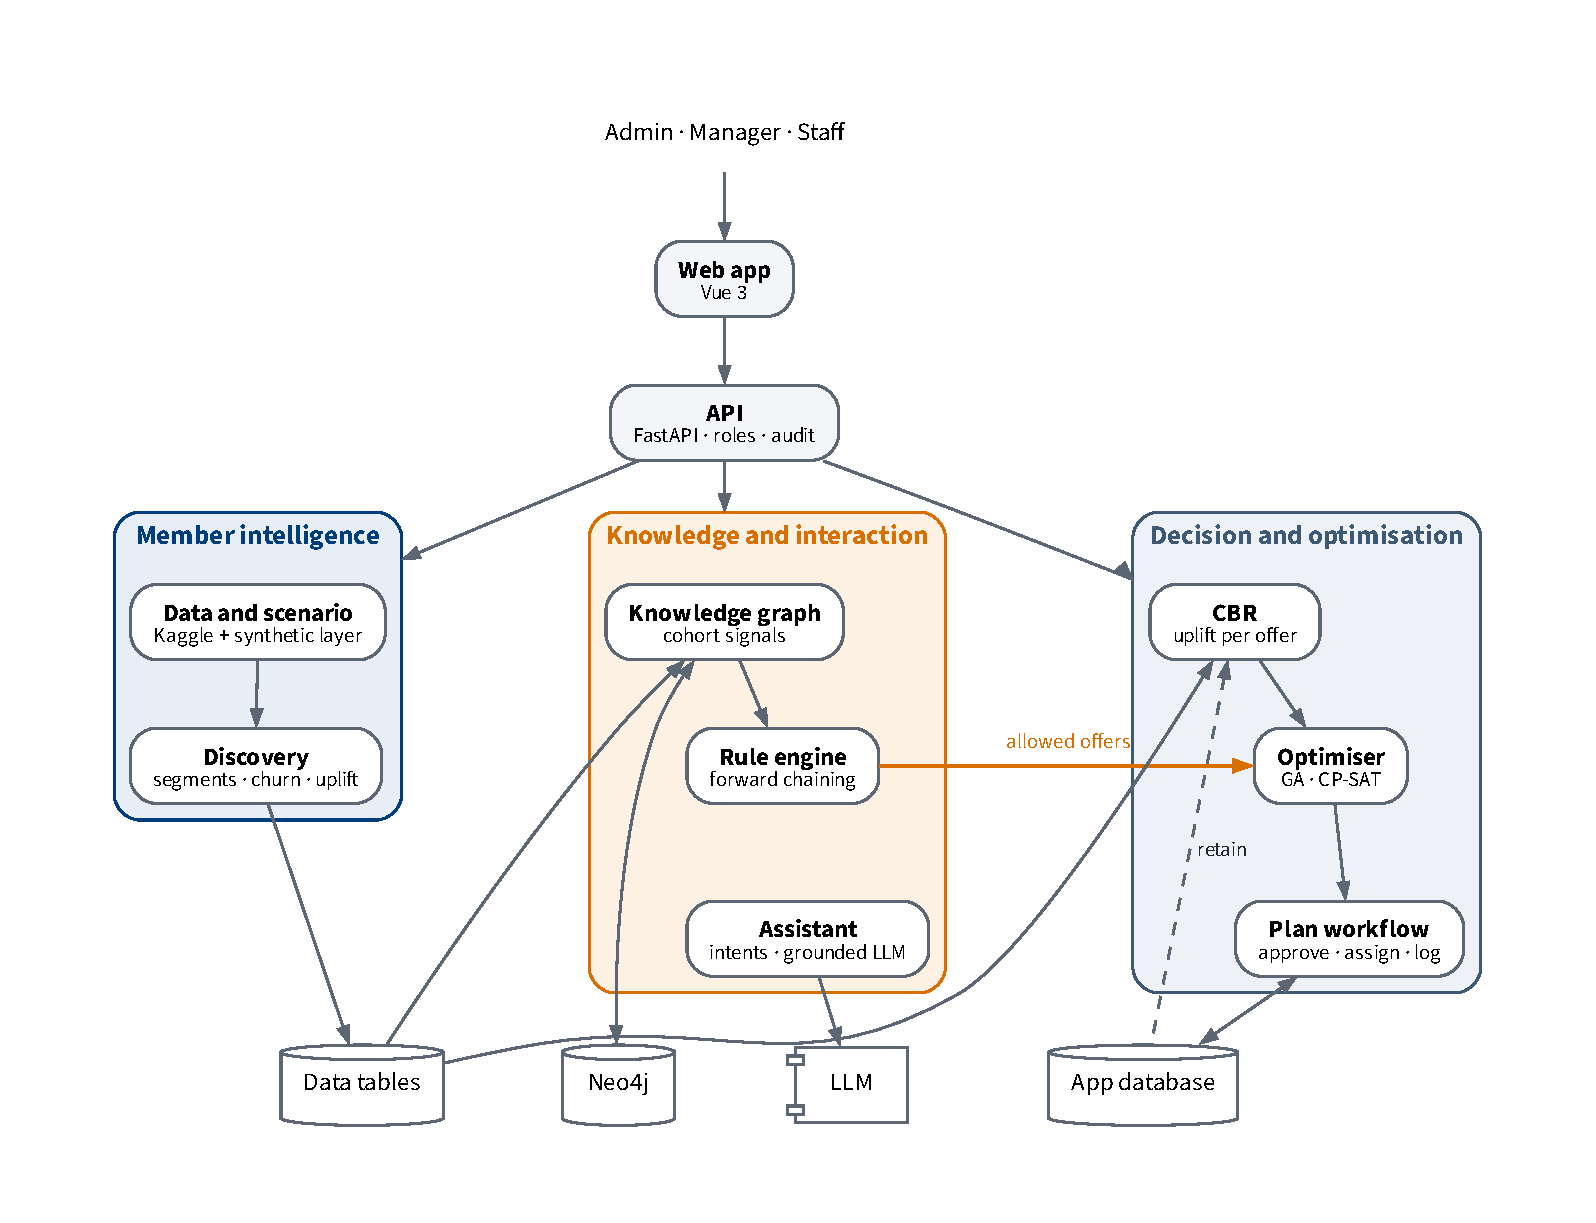
\includegraphics[width=0.74\linewidth]{diagrams/architecture.pdf}
  \caption{Architecture. Arrows show data flow; the dashed arrow is the learning loop through which logged outcomes return to the case base.}
  \label{fig:architecture}
\end{figure}

\begin{figure}[!htb]
  \centering
  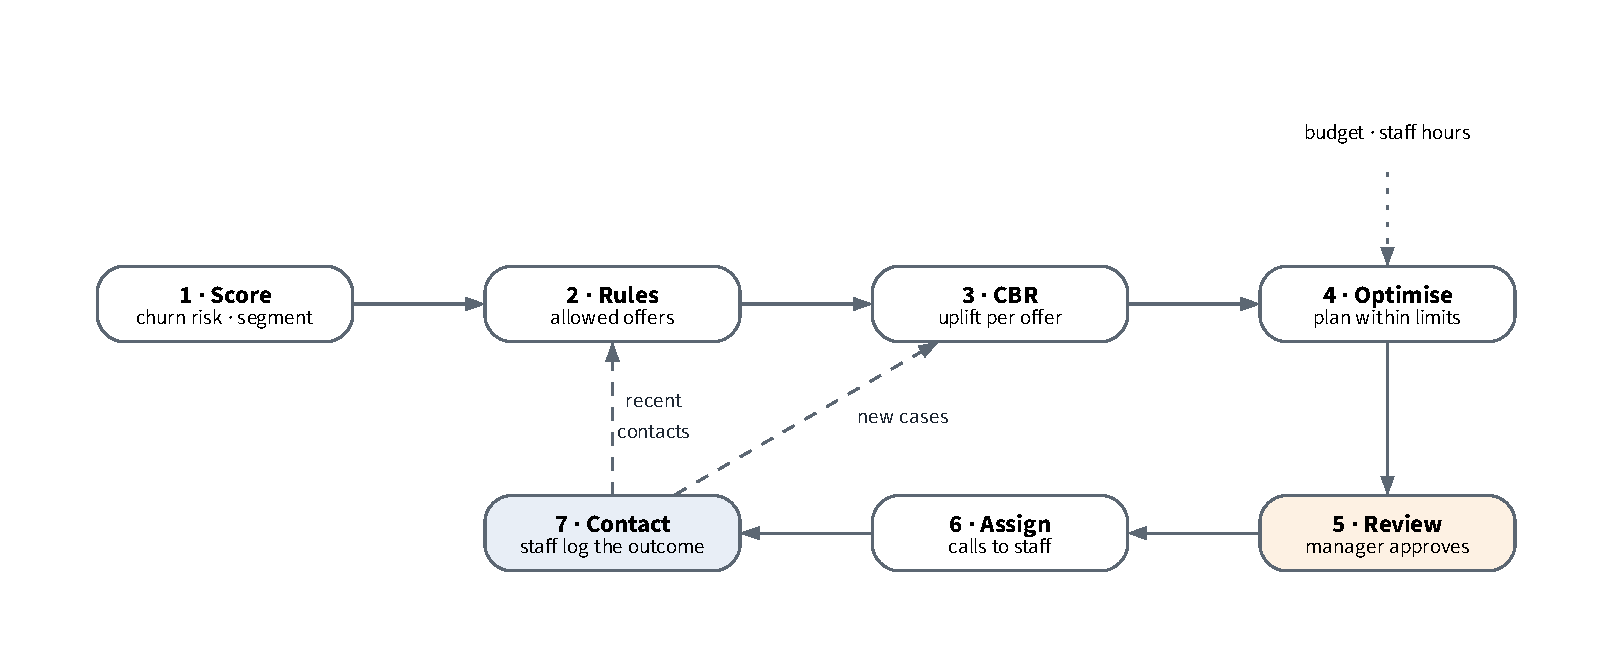
\includegraphics[width=0.92\linewidth]{diagrams/weekly-flow.pdf}
  \caption{The weekly cycle: steps 1--4 run automatically within the week's budget and staff hours; the manager reviews and approves, and staff contact members and log outcomes.}
  \label{fig:weekly}
\end{figure}

\section{Data and the scenario layer}
\label{sec:data}

Segmentation and churn prediction use only the 4,000 real members of the public \emph{Gym Customers Features and Churn} dataset~\cite{vinueza-gym}: 14 columns, 26.5\% churners, split 3,200/800 with stratification, and four derived features such as the visit trend (this month's visits over the lifetime rate), whose median is 0.69 for members who left and 1.00 for those who stayed (\cref{fig:trend}). Two same-month columns may leak the label, so E2 reports the model with and without them. The snapshot has no clubs, classes, offers or contact history, so a documented \emph{scenario layer} attaches a synthetic gym: three clubs, nine instructors and 18 classes consistent with each member's real visits; four offers with costs, staff minutes and stock; a heterogeneous ground-truth uplift for all 16,000 member--offer pairs (mean +5.8 points); two gym events (an instructor leaving and a class cancelled); and a randomised history of 2,400 past contacts (\cref{fig:scenario}). The ground truth is used only to grade, never by an estimator or planner. One command rebuilds every table, model and score in about 20 seconds from one seed.

\begin{figure}[!htb]
  \centering
  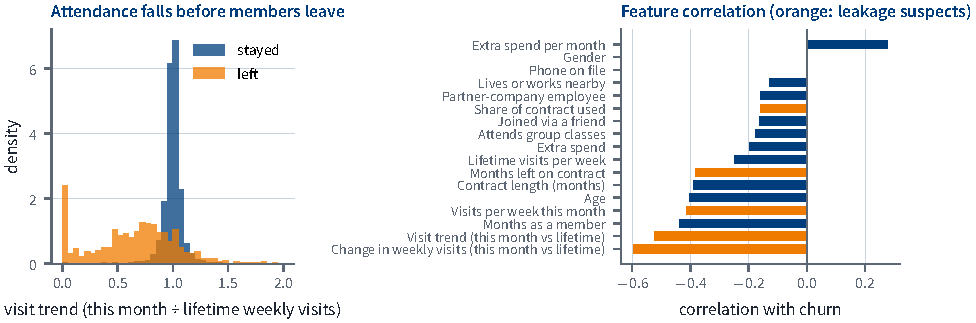
\includegraphics[width=\linewidth]{generated/trend_correlation.pdf}
  \caption{Left: the visit trend of members who stayed clusters at 1, while members who left spread below it, with a spike at 0 for those who did not come this month (medians 1.00 and 0.69). Right: correlation of each feature with churn; the two strongest are leakage suspects. Real Kaggle data.}
  \label{fig:trend}
  \source{\code{scripts/figures.py} (\code{trend}), as in \code{a_features_leakage.ipynb}, cells 2--4.}
\end{figure}
\begin{figure}[!htb]
  \centering
  \pgfplotstableread{\results{a5_true_uplift_by_segment.csv}}\upseg
  \begin{tikzpicture}
    \begin{axis}[anchorhbar, scale only axis, width=0.33\linewidth, height=4.4cm, bar width=3.6pt,
        ytick=data, yticklabels from table={\upseg}{segment}, y dir=reverse,
        enlarge y limits=0.16, xlabel={true uplift (percentage points)}, xmin=-5, xmax=26,
        legend style={at={(0.5,1.03)}, anchor=south, legend columns=2, /tikz/every even column/.append style={column sep=6pt}}, reverse legend,
        title={Effect by segment and offer}, title style={yshift=13mm}]
      \addplot[fill=cSky]    table[y expr=\coordindex, x expr=\thisrow{checkin_message}*100]{\upseg};
      \addplot[fill=cTeal]   table[y expr=\coordindex, x expr=\thisrow{class_pass}*100]{\upseg};
      \addplot[fill=cOrange] table[y expr=\coordindex, x expr=\thisrow{discount_1m}*100]{\upseg};
      \addplot[fill=cBlue]   table[y expr=\coordindex, x expr=\thisrow{free_pt_session}*100]{\upseg};
      \legend{Check-in message, Class pass, 20\% discount, Free PT session}
    \end{axis}
  \end{tikzpicture}\hfill
  \begin{tikzpicture}
    \begin{axis}[anchorhbar, scale only axis, width=0.24\linewidth, height=4.4cm, bar width=7pt, bar shift=0pt,
        symbolic y coords={All treated,Free PT session,Class pass,20\% discount,Check-in message,No contact},
        ytick={All treated,Free PT session,Class pass,20\% discount,Check-in message,No contact},
        y dir=reverse, enlarge y limits=0.11, xmin=60, xmax=80, xlabel={members who stayed (\%)},
        title={Intervention history}, title style={yshift=13mm}, clip=false,
        nodes near coords={\axisnum{\pgfplotspointmeta}}, nodes near coords style={font=\sffamily\scriptsize, text=navy},
        every node near coord/.append style={/pgf/number format/.cd, fixed, fixed zerofill, precision=1}]
      \addplot[fill=cGrey] coordinates {(67.0,No contact)};
      \addplot[fill=cBlue] coordinates {(67.8,Check-in message) (71.0,20\% discount) (71.2,Class pass) (77.6,Free PT session)};
      \addplot[fill=navy]  coordinates {(71.9,All treated)};
      \draw[cGrey, dashed, line width=0.6pt] (axis cs:67.0,No contact) -- (axis cs:67.0,All treated);
    \end{axis}
  \end{tikzpicture}
  \caption{The scenario's ground truth. Left: mean true uplift by segment and offer; a discount backfires on annual members. Right: share who stayed in each arm of the randomised history against the 984 controls (dashed).}
  \label{fig:scenario}
  \source{\code{results/a5_true_uplift_by_segment.csv}; \code{a_scenario_uplift.ipynb}.}
\end{figure}

\section{Methods}
\label{sec:methods}

\subsection{Member intelligence}

K-means~\cite{arthur2007kmeanspp} on seven behavioural features gives segments that staff can name; $k$ is chosen by a fixed rule on the silhouette~\cite{rousseeuw1987silhouettes} and names come from rules on the centres, so they survive a rebuild. Churn is predicted by the mean of a class-weighted logistic regression and LightGBM~\cite{ke2017lightgbm} over 17 features (\cref{fig:churnpipe}). Class weights matched SMOTE-NC~\cite{chawla2002smote} in cross-validation and were kept as simpler; a Platt calibrator~\cite{platt1999probabilistic} fitted on a held-out slice makes the probabilities honest, which matters because the planner multiplies them by uplift and value. Training members are scored out of fold, and each member's five drivers average the logistic-regression term with LightGBM's TreeSHAP value~\cite{lundberg2020trees} (\cref{fig:shap}). A T-learner~\cite{kunzel2019metalearners}, one outcome model per offer and one for controls, is the uplift benchmark.

\begin{figure}[!htb]
  \centering
  \begin{tikzpicture}[font=\sffamily\scriptsize,
      box/.style={draw=nusBlue, line width=0.6pt, rounded corners=2pt, fill=tint, align=center, minimum height=11mm, text width=23mm, text=ink},
      key/.style={box, fill=nusBlue, text=white, font=\sffamily\bfseries\scriptsize},
      outbox/.style={box, draw=nusOrange, fill=tintOrange},
      arr/.style={-{Latex[length=1.8mm]}, draw=muted, line width=0.6pt}]
    \node[box]    (f)    at (0,0)       {17 features\\13 Kaggle + 4 derived};
    \node[box]    (lr)   at (31mm,7.5mm)  {logistic regression\\class-weighted};
    \node[box]    (gb)   at (31mm,-7.5mm) {LightGBM\\300 trees, 15 leaves};
    \node[key]    (m)    at (62mm,0)    {mean of the two\\probabilities};
    \node[key]    (pl)   at (93mm,0)    {Platt calibration\\(640-member slice)};
    \node[outbox] (band) at (124mm,7.5mm)  {risk band\\high · medium · low};
    \node[outbox] (drv)  at (124mm,-7.5mm) {five drivers\\LR term + TreeSHAP};
    \coordinate (fs) at ($(f.east)!0.5!(lr.west|-f.east)$);
    \draw[arr] (f.east) -- (fs) |- (lr.west);
    \draw[arr] (fs) |- (gb.west);
    \coordinate (ms) at ($(lr.east|-m.west)!0.5!(m.west)$);
    \draw[draw=muted, line width=0.6pt] (lr.east) -| (ms);
    \draw[draw=muted, line width=0.6pt] (gb.east) -| (ms);
    \draw[arr] (ms) -- (m.west);
    \draw[arr] (m) -- (pl);
    \coordinate (ps) at ($(pl.east)!0.5!(band.west|-pl.east)$);
    \draw[draw=muted, line width=0.6pt] (pl.east) -- (ps);
    \draw[arr] (ps) |- (band.west);
    \draw[arr] (ps) |- (drv.west);
  \end{tikzpicture}
  \caption{The churn pipeline, fitted on 2,560 training members and calibrated on the remaining 640.}
  \label{fig:churnpipe}
\end{figure}

\begin{figure}[!htb]
  \centering
  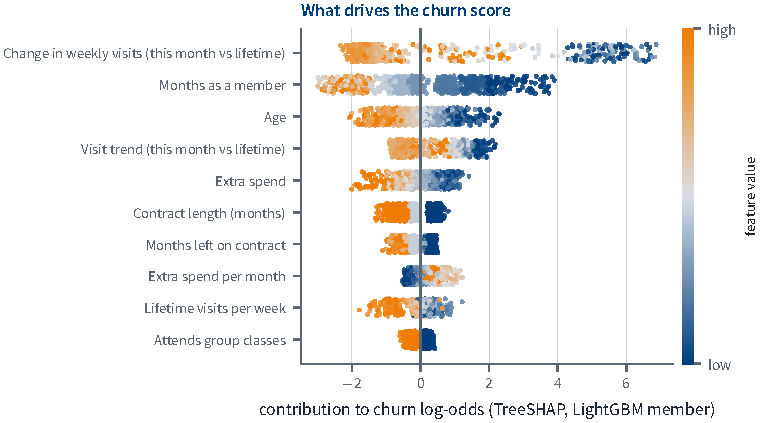
\includegraphics[width=0.66\linewidth]{generated/shap.pdf}
  \caption{TreeSHAP values of the LightGBM member on the 800 test members, for the ten most influential features. Each dot is a member, coloured by its feature value; dots to the right push towards churn. Real Kaggle data.}
  \label{fig:shap}
  \source{\code{scripts/figures.py} (\code{churn}), as in \code{a_churn.ipynb}, cell 5.}
\end{figure}
\subsection{Decision automation}

A forward-chaining engine~\cite{russell2021aima} runs 29 YAML rules: 8 \emph{derive} rules name patterns (falling regular, new member, routine disrupted), 16 \emph{playbooks} propose an offer on a channel, with twins for members without a phone, and 5 \emph{guardrails} block offers (contact and offer caps, eligibility, no paid offers at low risk, no repeat training session). Conflicts resolve by salience, specificity and order; each rule fires once, and blocks are applied after the loop, so guardrails always win. Every rule cites its source, a validator rejects inconsistent rule bases, and administrators edit, test, version and roll back rules in the application. Thresholds were drafted on the training data and adjusted after three \emph{simulated} manager interviews, which are disclosed as plausible opinion, not evidence.

\subsection{Decision and optimisation}

Each allowed member--offer--channel option is valued as $v_{mo} = \hat u_{mo} f_m H - c_o$, the estimated uplift~\cite{radcliffe2007uplift} times the monthly fee over a cautious six-month horizon, minus the offer's cost. The uplift comes from case-based reasoning~\cite{aamodt1994cbr} (\cref{fig:cbr}): retrieve the 200 nearest past cases in one shared neighbourhood of treated and untreated members, reuse it as a local A/B test, revise by empirical-Bayes shrinkage towards the offer's average~\cite{efron1975stein}, and retain logged outcomes as evidence but never in the averages, because the planner's own choices would bias them. A null test with shuffled offers rejected an earlier design that measured risk instead of effect. The plan maximises total value within budget, staff minutes, trainer minutes and stock, plus two effects between members who train together: \emph{spillover} and \emph{diminishing returns} per instructor. These make the problem non-linear, so a genetic algorithm (DEAP~\cite{fortin2012deap}) searches it with a repair operator and a greedy seed, while CP-SAT~\cite{ortools} solves the linear case exactly and benchmarks the full one on small instances. A policy evaluator grades plans against the true effects and is never used to choose one.

\begin{figure}[!htb]
  \centering
  % The case-based reasoner as a retrieve-reuse-revise-retain cycle; shared by both reports.
\begin{tikzpicture}[font=\sffamily\scriptsize,
    stage/.style={rectangle split, rectangle split parts=2, rectangle split part fill={nusBlue, white},
      draw=nusBlue, line width=0.6pt, text width=41mm, align=left, inner xsep=5pt, inner ysep=3.2pt,
      execute at begin node={\lefthyphenmin=64 \righthyphenmin=64 }},
    cyc/.style={-{Stealth[length=2.6mm, width=2.2mm]}, draw=nusOrange, line width=1.3pt},
    io/.style={-{Stealth[length=2.2mm, width=1.8mm]}, draw=muted, line width=0.7pt},
    iolab/.style={font=\sffamily\scriptsize, text=muted, align=center},
    link/.style={-{Stealth[length=1.8mm, width=1.5mm]}, draw=nusOrange!75, line width=0.7pt, dash pattern=on 2.2pt off 1.6pt},
    linklab/.style={font=\sffamily\tiny, text=nusOrange!85!black, fill=white, inner sep=1pt}]
  \newcommand{\stephead}[2]{\textcolor{white}{\bfseries\small #1\enskip #2}}
  \node[stage] (ret) at (-34mm, 19mm) {\stephead{1}{Retrieve}\nodepart{two}\color{ink}the 200 nearest past cases on 17 features, in one shared neighbourhood of treated and untreated members};
  \node[stage] (reu) at ( 34mm, 19mm) {\stephead{2}{Reuse}\nodepart{two}\color{ink}a local A/B test: the kernel-weighted stay rate with the offer minus the rate without it};
  \node[stage] (rev) at ( 34mm,-19mm) {\stephead{3}{Revise}\nodepart{two}\color{ink}empirical-Bayes shrinkage of the noisy local estimate towards the offer's average effect};
  \node[stage] (rtn) at (-34mm,-19mm) {\stephead{4}{Retain}\nodepart{two}\color{ink}each logged outcome becomes a new case, used as evidence but never in the offer averages};
  \node[circle, draw=nusOrange, line width=1pt, fill=tintOrange, minimum size=19mm, inner sep=0pt, align=center, text=ink] (cb) at (0,0)
    {\bfseries\small Case base\\[2pt]\mdseries\tiny 2,400 randomised\\[-1pt]\tiny cases + outcomes};
  \draw[cyc] (ret.east) -- (reu.west);
  \draw[cyc] (reu.south) -- (rev.north);
  \draw[cyc] (rev.west) -- (rtn.east);
  \draw[cyc] (rtn.north) -- (ret.south);
  \draw[link] (cb.135) -- node[linklab, sloped] {read} (ret.south east);
  \draw[link] (rtn.north east) -- node[linklab, sloped] {write} (cb.225);
  \draw[io] ([xshift=-16mm]ret.west) -- node[iolab, above=1pt] {member\\and offer} (ret.west);
  \draw[io] ([xshift=-16mm]rtn.west) -- node[iolab, above=1pt] {outcome\\logged} (rtn.west);
  \draw[io] (rev.east) -- node[iolab, above=1pt] {estimate +\\precedents} ([xshift=16mm]rev.east);
\end{tikzpicture}

  \caption{The case-based reasoner. The neighbours that produce an estimate are shown to staff as its precedents.}
  \label{fig:cbr}
\end{figure}

\subsection{Knowledge graph and staff assistant}

A Neo4j knowledge graph~\cite{hogan2021kg} links members, classes, instructors, clubs, offers and events through read-only parameterised Cypher. It flags members whose anchor instructor left or whose class was cancelled, as rule facts cached so the rules work without Neo4j; it gives the optimiser its class cohorts; and it simulates an event's impact without changing data (\cref{fig:kgsim}). The staff assistant routes a question to one of seven intents with sentence-embedding centroids~\cite{reimers2019sbert} and an \enquote{unknown} threshold, fills slots, runs one deterministic tool, and lets the language model only phrase the numbered evidence with citations, or answer that it does not know (\cref{fig:assistantpipe,fig:assistant}). Without the model, it returns the cited evidence itself.

\begin{figure}[!htb]
  \centering
  \begin{tikzpicture}[font=\sffamily\scriptsize,
      st/.style={draw=nusBlue, line width=0.6pt, rounded corners=2pt, fill=tint, align=center, minimum height=11mm, text width=21mm, text=ink},
      llm/.style={st, draw=nusOrange, fill=tintOrange},
      arr/.style={-{Latex[length=1.8mm]}, draw=muted, line width=0.6pt}]
    \node[st]  (q)  at (0,0)        {\textbf{question}\\+ member on page};
    \node[st]  (i)  at (26.5mm,0)   {\textbf{intent}\\embedding centroid, threshold 0.35};
    \node[st]  (s)  at (53mm,0)     {\textbf{slots}\\ids, amounts, names, filters};
    \node[st]  (t)  at (79.5mm,0)   {\textbf{tool}\\one deterministic function per intent};
    \node[st]  (e)  at (106mm,0)    {\textbf{evidence}\\numbered lines [E1], [E2]…};
    \node[llm] (l)  at (132.5mm,0)  {\textbf{LLM}\\phrases and cites, or says it does not know};
    \foreach \a/\b in {q/i, i/s, s/t, t/e, e/l} \draw[arr] (\a) -- (\b);
  \end{tikzpicture}
  \caption{The assistant pipeline: the language model never chooses a tool and never sees data a tool did not return.}
  \label{fig:assistantpipe}
\end{figure}

\begin{figure}[!htb]
  \centering
  \begin{subfigure}[t]{0.495\linewidth}
    \screenshot[\linewidth]{screens/graph-content.png}
    \caption{Simulating instructor Maya Chen leaving: 312 members affected, 54 at high risk, with her neighbourhood.}
    \label{fig:kgsim}
  \end{subfigure}\hfill
  \begin{subfigure}[t]{0.495\linewidth}
    \screenshot[\linewidth]{screens/assistant-content.png}
    \caption{The assistant answering about member M1460 with the local \code{qwen2.5:7b-instruct} model, citing its sources.}
    \label{fig:assistant}
  \end{subfigure}
  \caption{The knowledge graph and the staff assistant in the application.}
\end{figure}
\section{System development and implementation}
\label{sec:impl}

One command builds the data and models, migrates and seeds the database with a demo week, and loads the graph. Sixteen pages serve three roles (\cref{fig:screens}): managers work from the dashboard, plan and scenarios; staff from a call sheet with talking points, message drafts and two-tap outcome logging; administrators from versioned rules, offers, data and models, users and an audit log of every write. Member~360 shows every component's reasoning about one member on one screen. Risk is always shown as text and colour; planning continues when Neo4j or the language model is down; and 195 offline tests guard against leakage, infeasible plans, rule order, unsafe queries and role or audit errors.

\begin{figure}[!htb]
  \centering
  \screenshot[\linewidth]{screens/dashboard.png}\par\medskip
  \begin{subfigure}[t]{0.495\linewidth}
    \screenshot[\linewidth]{screens/member360-content.png}
    \caption{Member 360: risk, drivers, profile and rule trace for one member.}
  \end{subfigure}\hfill
  \begin{subfigure}[t]{0.495\linewidth}
    \screenshot[\linewidth]{screens/plan-content.png}
    \caption{The weekly plan: 182 approved contacts, each with a reason.}
  \end{subfigure}
  \caption{The application on the demo data. Top: the manager's dashboard.}
  \label{fig:screens}
\end{figure}

\FloatBarrier
\section{Experiments and findings}
\label{sec:exp}

E1 and E2 use only real members; E3--E7 are graded by the scenario's ground truth, which no estimator or planner reads; E8 evaluates the assistant on the system's own evidence (\cref{tab:exp}).

\begin{table}[!htb]
  \caption{The eight experiments: real-data experiments use the 4,000 Kaggle members; scenario experiments are graded against the synthetic ground truth.}
  \label{tab:exp}
  \begin{tabularx}{\linewidth}{@{}l L L l@{}}
    \toprule
    & \hd{Question} & \hd{Key result} & \hd{Verdict} \\
    \midrule
    E1 & meaningful segments? \databadge{real} & $k=4$ by rule; stability ARI 1.00; churn from 94.6\% to 1.4\% & \verdict{met} \\
    E2 & churn model beats simple rules? \databadge{real} & F1 0.908, PR-AUC 0.973, Brier 0.035 vs 0.862 / 0.953 / 0.056 (logistic) and 0.549 / 0.390 / 0.336 (visit rule) & \verdict{met} \\
    E3 & who is persuadable? \databadge{scenario} & CBR ties the T-learner (Spearman 0.39 each), better for PT and discount & \verdict{partly} \\
    E4 & more members per dollar? \databadge{scenario} & 22--138\% more members kept than by risk or schedule; 0 of 198 plans infeasible & \verdict{met} \\
    E5 & GA good and fast enough? \databadge{scenario} & within 0.24\% of the optimum on small instances; 33\,s for 2,000 members & \verdict{partly} \\
    E6 & rules correct; guardrails matter? \databadge{scenario} & 0 validator issues; 29 of 29 cases; guardrails remove 31.3\% of proposals & \verdict{met} \\
    E7 & graph signals add information? \databadge{scenario} & no ranking gain; 243 extra low-risk members reached; +7 members at 120\,h & \verdict{partly} \\
    E8 & assistant accurate, grounded? \databadge{scenario} & 96.2\% of sentences supported; held-out routing 50.0\% vs 54.2\% for keywords & \verdict{partly} \\
    \bottomrule
  \end{tabularx}
  \source{\code{SystemCode/notebooks/results/}; full method and caveats per experiment in the full report.}
\end{table}

\paragraph{Segments and churn (E1, E2).} Silhouette is low and flat on behavioural data, but the four segments are stable across seeds and separate churn by a factor of almost 70 (\cref{fig:e1}); the 728 \enquote{new and slipping} members hold about two-thirds of all churners. The calibrated ensemble beats both baselines on every metric (\cref{fig:e2}); each risk band churns at about its predicted rate (high band 93.9\% against 95.1\% predicted), and without the two suspect same-month columns F1 falls to 0.817, the honest lower bound. Recall for the rare churners aged 31 and over is 0.52, which we report with a mitigation rather than hide.

\begin{figure}[!htb]
  \centering
  \pgfplotstableread{\results{e1_silhouette_by_k.csv}}\sil
  \pgfplotstableread{\results{e1_segment_profiles.csv}}\seg
  \begin{tikzpicture}
    \begin{axis}[anchor, scale only axis, width=0.36\linewidth, height=4.1cm, xlabel={number of segments \textit{k}},
        ylabel={silhouette}, ymin=0.15, ymax=0.182, xtick={2,...,10}, title={Silhouette on the training split},
        yticklabel style={/pgf/number format/fixed, /pgf/number format/precision=3}]
      \fill[nusOrange!12] (axis cs:3,0.1688) rectangle (axis cs:8,0.1776);
      \addplot[cBlue, mark=*, mark size=1.6pt] table[x index=0, y=silhouette]{\sil};
      \draw[nusOrange, dashed, line width=0.8pt] (axis cs:4,0.15) -- (axis cs:4,0.182);
      \node[font=\sffamily\tiny, text=nusOrange, anchor=south west] at (axis cs:4.1,0.151) {chosen \textit{k} = 4};
    \end{axis}
  \end{tikzpicture}\hfill
  \begin{tikzpicture}
    \begin{axis}[anchorhbar, scale only axis, width=0.3\linewidth, height=4.1cm, bar width=9pt,
        ytick=data, yticklabels from table={\seg}{name}, y dir=reverse, enlarge y limits=0.18,
        xmin=0, xmax=100, xlabel={churn rate (\%)}, title={Churn by segment (size)},
        nodes near coords={\axisnum[fixed, precision=1]{\pgfplotspointmeta}\,\%},
        nodes near coords style={font=\sffamily\scriptsize, text=ink}, point meta=x]
      \addplot[fill=cBlue] table[y expr=\coordindex, x expr=\thisrow{churn_rate}*100]{\seg};
    \end{axis}
  \end{tikzpicture}
  \caption{E1. Left: silhouette is low and nearly flat; the shaded band is within 5\% of the best $k$ between 3 and 8, and the rule picks the most detailed $k$ inside it. Right: the four segments separate churn from 94.6\% to 1.4\% (sizes 728, 1,365, 961 and 946).}
  \label{fig:e1}
  \source{\code{results/e1_silhouette_by_k.csv}, \code{results/e1_segment_profiles.csv}; \code{a_segmentation.ipynb}.}
\end{figure}
\begin{figure}[!htb]
  \centering
  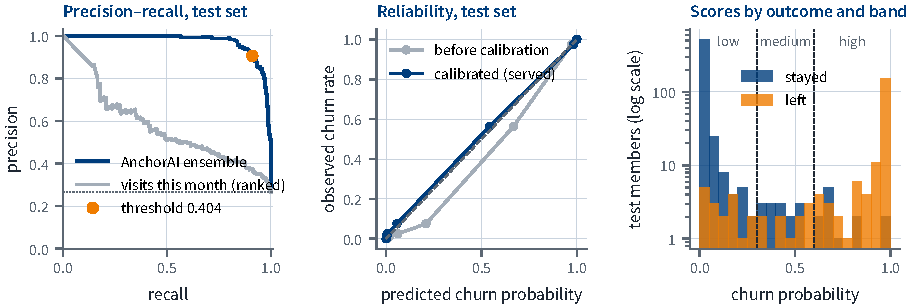
\includegraphics[width=\linewidth]{generated/churn_evaluation.pdf}
  \caption{E2 on the 800 test members: precision--recall against ranking by this month's visits, reliability before and after calibration, and scores by outcome with the band cut-offs.}
  \label{fig:e2}
\end{figure}

\paragraph{Uplift and plans (E3--E5).} Case-based reasoning matches the T-learner overall and is better where effects are large (\cref{fig:e3}), but cannot rank members for the small-effect check-in and class pass, which costs 3.7 members a week at the default 36 staff hours (21.0 against 24.6 extra members; level or ahead with more staff time). Planning by effect keeps 1.9 to 3.5 times as many members as contacting by schedule or risk with perfect knowledge (\cref{fig:e4}) and 22--138\% more on estimates. On noisy CBR estimates, however, the genetic algorithm keeps fewer members than greedy: the optimiser's curse~\cite{smith2006curse}, where stronger search selects estimates that happen to be too high. On its own objective the algorithm is near-optimal (0.8--2.3\% from CP-SAT's optimum on the linear problem; within 0.24\% on small full instances) and robust to the assumed spillover and diminishing-returns strengths, but CP-SAT is the better tool for the linear problem.

\begin{figure}[!htb]
  \centering
  \pgfplotstableread{\results{e3_uplift_vs_truth.csv}}\upl
  \begin{tikzpicture}
    \begin{axis}[anchorbar, scale only axis, width=0.5\linewidth, height=4.2cm, bar width=5.5pt,
        ymin=-0.05, ymax=1, ylabel={Spearman with true uplift},
        xtick={0,...,4}, xticklabels={Check-in, Class pass, Discount, Free PT, All pairs},
        unbounded coords=discard, title={Ranking quality by offer}, title style={yshift=11pt}, enlarge x limits=0.13, ytick={0,0.25,...,1},
        legend style={at={(0.5,1.02)}, anchor=south, legend columns=4, /tikz/every even column/.append style={column sep=5pt}}]
      \addplot[fill=cBlue]   table[x expr=\coordindex,    y=spearman, skip coords between index={5}{20}]{\upl};
      \addplot[fill=cOrange] table[x expr=\coordindex-5,  y=spearman, skip coords between index={0}{5}, skip coords between index={10}{20}]{\upl};
      \addplot[fill=cSky]    table[x expr=\coordindex-10, y=spearman, skip coords between index={0}{10}, skip coords between index={15}{20}]{\upl};
      \addplot[fill=cGrey]   table[x expr=\coordindex-15, y=spearman, skip coords between index={0}{15}]{\upl};
      \legend{CBR, T-learner, churn risk, random}
    \end{axis}
  \end{tikzpicture}\hfill
  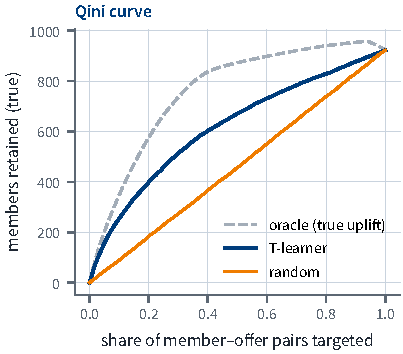
\includegraphics[width=0.4\linewidth]{generated/qini.pdf}
  \caption{E3. Left: rank correlation between estimated and true uplift; CBR gives every member the offer's average for the check-in and the class pass, so it has no ranking there. Right: Qini curve of the T-learner against the oracle and random targeting.}
  \label{fig:e3}
  \source{\code{results/e3_uplift_vs_truth.csv}, \code{results/a6_tlearner_recovery.csv}; \code{b_cbr.ipynb}, \code{a_scenario_uplift.ipynb}.}
\end{figure}
\begin{figure}[!htb]
  \centering
  \begin{tikzpicture}
    \begin{axis}[anchorbar, width=\linewidth, height=4.3cm, bar width=6.5pt,
        symbolic x coords={36 h \$1.5k, 72 h \$1.5k, 72 h \$4k, 120 h \$1.5k, 120 h \$4k}, xtick=data,
        ymin=0, ymax=80, ylabel={extra members kept}, enlarge x limits=0.1,
        legend style={at={(0.02,0.98)}, anchor=north west, legend columns=4, /tikz/every even column/.append style={column sep=6pt}},
        nodes near coords={\axisnum{\pgfplotspointmeta}}, nodes near coords style={font=\sffamily\tiny, text=ink, rotate=90, anchor=west},
        every node near coord/.append style={/pgf/number format/.cd, fixed, fixed zerofill, precision=1}]
      \addplot[fill=cGrey]   coordinates {(36 h \$1.5k,10.4) (72 h \$1.5k,20.1) (72 h \$4k,20.2) (120 h \$1.5k,20.1) (120 h \$4k,20.2)};
      \addplot[fill=cSky]    coordinates {(36 h \$1.5k,13.7) (72 h \$1.5k,21.0) (72 h \$4k,21.4) (120 h \$1.5k,21.0) (120 h \$4k,21.4)};
      \addplot[fill=cOrange] coordinates {(36 h \$1.5k,28.8) (72 h \$1.5k,44.5) (72 h \$4k,50.1) (120 h \$1.5k,47.6) (120 h \$4k,64.1)};
      \addplot[fill=cBlue]   coordinates {(36 h \$1.5k,32.5) (72 h \$1.5k,45.7) (72 h \$4k,54.0) (120 h \$1.5k,47.6) (120 h \$4k,70.8)};
      \legend{contact-all, risk-top-\textit{k}, greedy-uplift, genetic algorithm}
    \end{axis}
  \end{tikzpicture}
  \caption{E4 with perfect knowledge: extra members kept by each planner, by staff hours and weekly budget.}
  \label{fig:e4}
  \source{\code{results/e4_optimiser.csv}, mean over three seeds.}
\end{figure}

\paragraph{Rules, graph and assistant (E6--E8).} The rule base is consistent, and its guardrails remove 31.3\% of proposals, almost all repeat contacts within 30 days, at little cost where staff time binds; the scenario has no fatigue effect, so we claim safety, not retention. The graph's flags recover the designed event effects (hazard ×1.80 and ×1.32) but do not improve the risk ranking; they route 243 low-risk members with a disrupted routine to a free check-in, worth about 7 members when staff time allows. The assistant states only what its evidence supports (no invented number; 15 of 17 answers fully supported), but on 24 questions written by team members who never saw its training examples it routes no better than a keyword router (\cref{fig:e8}), mostly by answering off-topic questions instead of refusing.

\begin{figure}[!htb]
  \centering
  \pgfplotstableread{\results{e8_threshold_sweep.csv}}\sw
  \begin{tikzpicture}
    \begin{axis}[anchor, scale only axis, width=0.4\linewidth, height=3.3cm, xlabel={similarity threshold for \enquote{unknown}},
        ylabel={share}, ymin=0, ymax=1, title={Threshold trade-off (86 questions)},
        legend style={at={(0.98,0.5)}, anchor=east}, xticklabel style={/pgf/number format/fixed, /pgf/number format/precision=2}]
      \draw[muted, dashed, line width=0.6pt] (axis cs:0.35,0) -- (axis cs:0.35,1);
      \addplot[cBlue] table[x=threshold, y=accuracy]{\sw};
      \addplot[cOrange] table[x=threshold, y=off_topic_answered]{\sw};
      \addplot[cSky] table[x=threshold, y=in_scope_refused]{\sw};
      \legend{accuracy, off-topic answered, in-scope refused}
    \end{axis}
  \end{tikzpicture}\hfill
  \begin{minipage}[b]{0.46\linewidth}
    \small\sffamily
    \begin{tabular*}{\linewidth}{@{\extracolsep{\fill}}l r S[table-format=2.1] S[table-format=2.1]@{}}
      \toprule
      \hd{Questions} & \hd{n} & {\hd{Classifier}} & {\hd{Keywords}} \\
      \midrule
      AI-written & 62 & \bfseries 91.9 & 77.4 \\
      Held out & 24 & 50.0 & \bfseries 54.2 \\
      \bottomrule
    \end{tabular*}
    \par\vspace{3pt}{\scriptsize\color{muted}Intent accuracy (\%).}\par\vspace{8pt}
  \end{minipage}
  \caption{E8: raising the threshold refuses more off-topic questions but also more in-scope ones; on held-out questions the classifier is no better than keywords.}
  \label{fig:e8}
  \source{\code{results/e8_threshold_sweep.csv}, \code{results/e8_intent_predictions.csv}.}
\end{figure}

\FloatBarrier
\section{Findings, discussion and future work}
\label{sec:conclusions}

\paragraph{Findings.} AnchorAI shows that a gym's weekly retention decision can be automated and explained end to end. Real data supports a calibrated churn model and interpretable segments, with most churn in one recognisable group of new members whose visits are falling. Planning by estimated effect keeps substantially more members than planning by risk, but the quality of the uplift estimates, not the strength of the search, limits the planner. The rules and graph add safety and reach rather than accuracy, and the assistant is faithful to its evidence but routes unseen questions no better than keywords.

\paragraph{Discussion.} The limits are as clear as the results. The effects that grade the plans are synthetic and grow with risk by design; the real data is one undated snapshot, so leakage of the same-month columns cannot be settled; the interviews were simulated and no gym staff used the system; and the assistant's held-out set is small. An operator should act on new members whose visits fall, review older medium-risk members by hand, keep visit dates and contact outcomes, and hold back a small random control group each week, preferring the greedy planner until better estimates exist.

\paragraph{Future work.} Time-stamped data and randomised contacts to learn real effects; uncertainty-aware planning that stops a strong optimiser amplifying noisy estimates; out-of-scope detection for the assistant; drift monitoring after each rebuild; and a field study with gym staff.

\printbibliography[heading=bibintoc, title=References]

\clearpage
\renewcommand{\thesection}{\Alph{section}}
\setcounter{section}{0}
\addtocontents{toc}{\protect\smallskip}

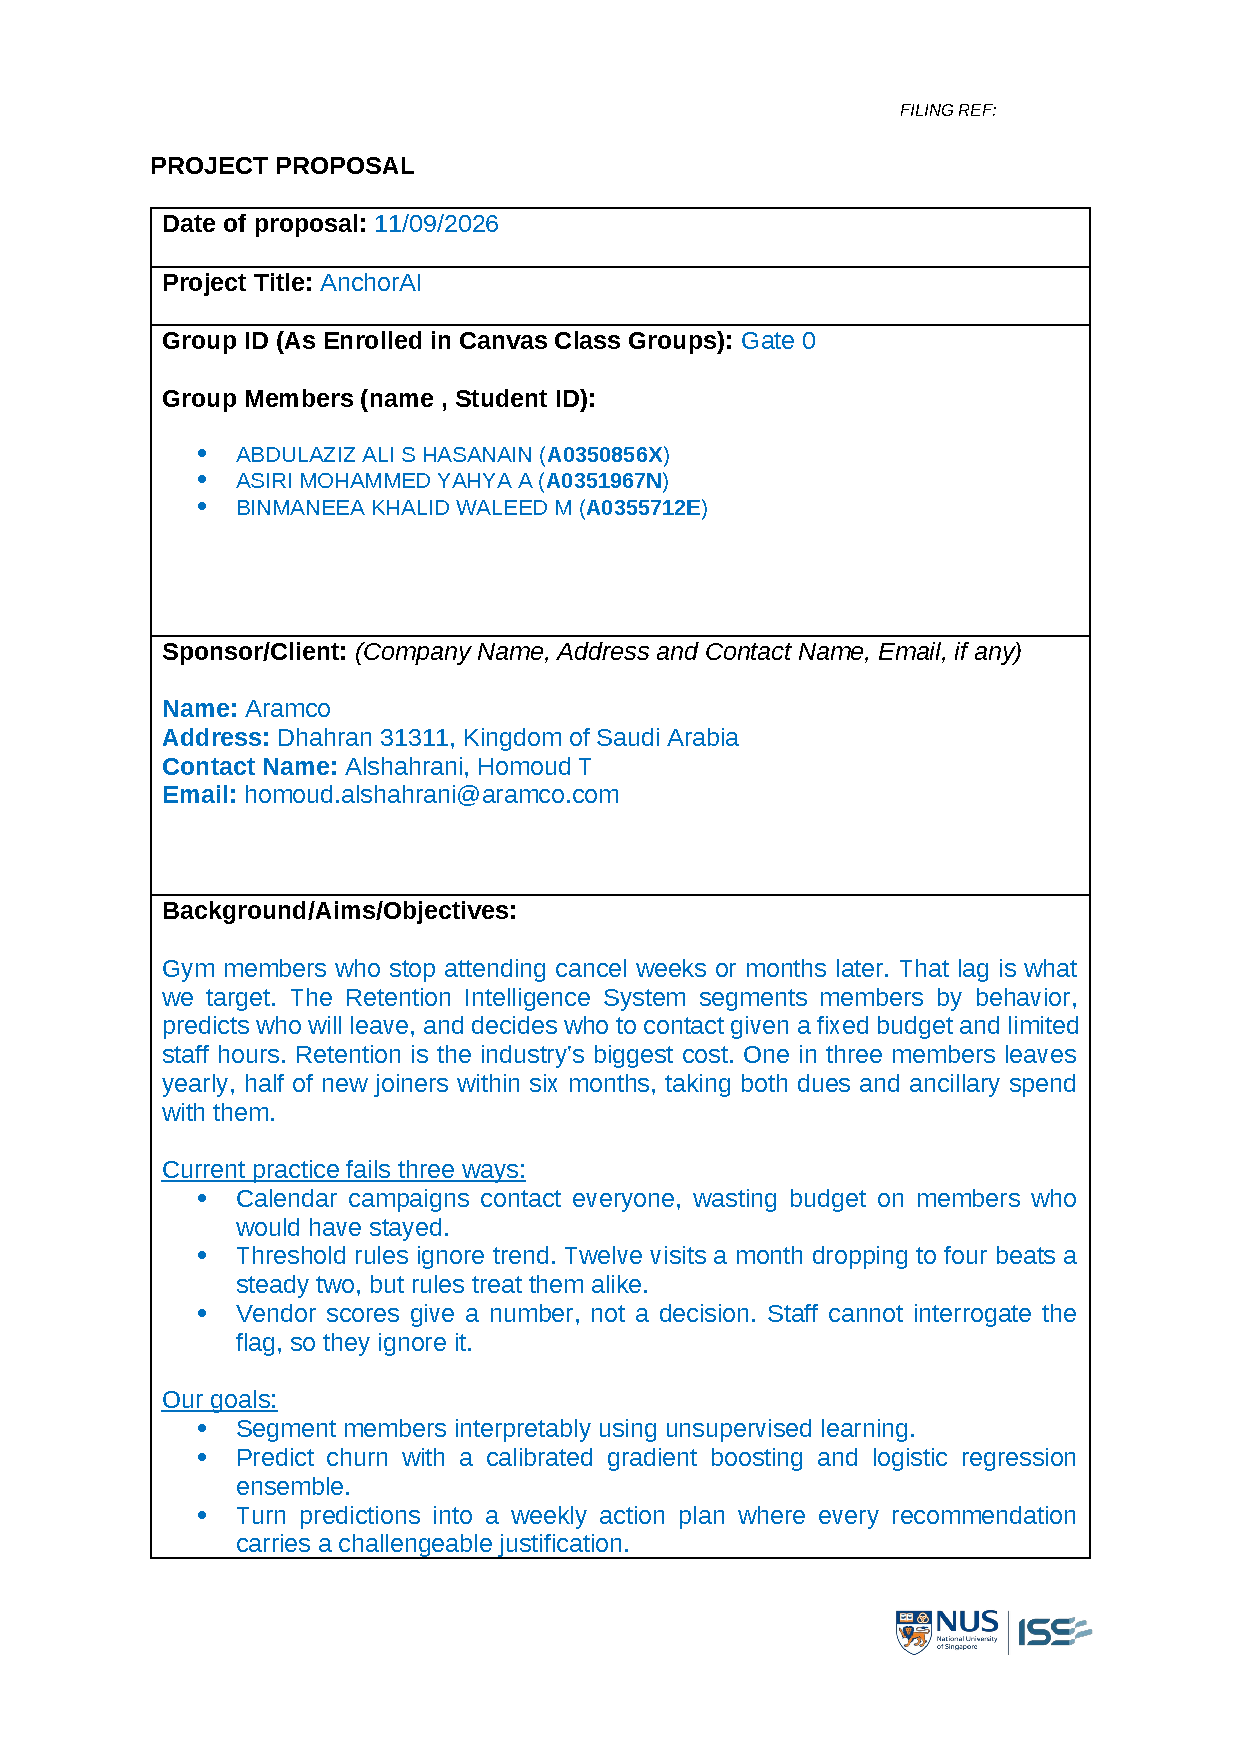
\includepdf[pages=1, scale=0.74, offset=0 -14mm, frame,
  pagecommand={\section{Project proposal}\label{app:proposal}\vspace{-0.4\baselineskip}{\small The proposal as submitted on 11 September 2026; pages 1--3 of the original, the fourth being blank.}}]{figures/appendix/proposal.pdf}
\includepdf[pages=2-3, scale=0.8, frame, pagecommand={\thispagestyle{scrheadings}}]{figures/appendix/proposal.pdf}

\section{Mapping to MR, RS and CGS}
\label{app:mapping}

All four technique groups the module requires are covered: decision automation, resource optimisation, knowledge discovery and cognitive systems (MR Machine Reasoning, RS Reasoning Systems, CGS Cognitive Systems; D is the course day). The full report also lists every change from the proposal and its reason.

% MR / RS / CGS mapping table, shared by both reports
{\small\sffamily
\begin{xltabular}{\linewidth}{@{}P{0.2\linewidth} L l P{0.2\linewidth}@{}}
  \caption{Techniques as built, by course and evidence.}\label{tab:mapping}\\
  \toprule
  \hd{Component} & \hd{Technique as built} & \hd{Course} & \hd{Evidence} \\
  \midrule
  \endfirsthead
  \toprule
  \hd{Component} & \hd{Technique as built} & \hd{Course} & \hd{Evidence} \\
  \midrule
  \endhead
  Data preparation & stratified split; SMOTE-NC inside folds compared with class weights; CRISP-DM & RS D2 & E2 \\
  Features & trend and ratio features, scaling, leakage check & MR D4, RS D2 & E2, leakage check \\
  Segmentation & K-means, silhouette, stability (adjusted Rand index), profiles & MR D4 & E1 \\
  Churn model & class-weighted logistic regression and LightGBM ensemble, Platt calibration; F1, PR-AUC, Brier & MR D2, D4 & E2 \\
  Driver explanations & averaged logistic-regression terms and TreeSHAP contributions per member & MR D3, D4 & E2 drivers \\
  Scenario layer & synthetic gym and randomised history with known effects & MR D3 & scenario layer \\
  Uplift baseline & T-learner (self-researched) & MR D4 & E3 \\
  Offer reasoner & case-based reasoning: retrieve, reuse, revise (shrinkage), retain & MR D2 & E3 \\
  Plan optimiser & genetic algorithm with repair, elitism, spillover and diminishing returns & RS D4 & E4, E5 \\
  Exact benchmark & CP-SAT constraint optimisation & MR D1, RS D1 & E5 \\
  Policy evaluation & simulation-based comparison against three baselines & RS D1 & E4 \\
  Rule engine & forward chaining over derive, playbook and guardrail rules; salience; traces; versions & MR D2, RS D1 & E6 \\
  Knowledge graph & Neo4j and Cypher; multi-hop cohort signals; read-only parameterised queries & MR D3, RS D5 & E7 \\
  Intent detection & sentence-embedding centroids with an unknown threshold; slot filling & CGS D1 & E8 \\
  Grounded generation & deterministic tool, then an LLM phrases cited evidence only & CGS D1, D3 & E8 \\
  Assistant evaluation & keyword baseline; static checks; calibrated LLM-as-judge; local and hosted models & CGS D2, D3 & E8 \\
  Message drafts & LLM drafts with a rule check and a template fallback & CGS D1 & drafts in the application \\
  Overall & hybrid machine learning, rules, optimisation, knowledge graph and language interface with human review & RS D1, CGS D1 & E4, E6, E7 \\
  \bottomrule
\end{xltabular}}


\clearpage
\section{Installation and user guide}
\label{app:install}

\paragraph{Install.} Prerequisites: Git, uv 0.13+, Node.js 20+, Docker with Compose, and optionally an OpenAI-compatible LLM endpoint (the default is a local Ollama \code{qwen2.5:7b-instruct}). Download \emph{Gym Customers Features and Churn} from Kaggle~\cite{vinueza-gym} into \code{SystemCode/data/raw/}; the data is CC BY-NC-SA 4.0 and not redistributed.
\begin{shell}
git clone <repo-url> AnchorAI && cd AnchorAI
cp .env.example .env                  # set ANCHORAI_JWT_SECRET and LLM_*
docker compose up -d neo4j            # knowledge graph
cd SystemCode/backend && uv sync
uv run anchorai setup                 # data, models, seeded DB, graph
uv run uvicorn anchorai.api.main:app  # API on :8000
cd ../frontend && npm install
npm run dev                           # web app on http://localhost:5173
\end{shell}
Sign in as \code{admin}, \code{manager}, \code{staff1} or \code{staff2} with the password \code{anchorai}. The pipeline, API and web application run without Neo4j or a language model, with the graph panels and assistant shown as unavailable. \code{uv run pytest -q} runs the 195 offline tests; \code{uv run anchorai db reset} restores the demo database; the administrator's Settings page checks every service.

\paragraph{Manager.} The \emph{Dashboard} shows members at high risk, revenue at risk, plan coverage and last week's outcomes (\cref{fig:screens}). On \emph{Weekly plan}, set the budget and staff hours, choose a planner (genetic algorithm, exact or greedy) and select \emph{Generate plan}. \emph{Why} on a row opens the member's drivers, rule trace, gym events and similar past members. Remove, add or swap contacts with a reason (each is rule-checked at once), \emph{Re-optimise the rest}, then \emph{Approve plan}: contacts are assigned to staff by hours and skills, with printable call sheets. \emph{Scenarios} compares five planners on a what-if budget; \emph{Events \& roster} records departures and cancellations; \emph{Knowledge graph} simulates an event without changing data.

\paragraph{Staff.} \emph{My contacts} lists this week's assigned members in priority order with the offer, channel, reason and talking points. Log each outcome in two taps (accepted, declined, reached, follow-up, no answer); \emph{Draft message} writes an editable message that is never sent automatically. \emph{Member 360} and the \emph{Assistant} answer questions from AnchorAI's own data, with evidence chips behind every sentence.

\paragraph{Administrator.} \emph{Rules} edits, tests on any member, versions and rolls back the rule base; \emph{Offers \& constraints} sets the catalogue, staff hours and skills, budget and contact caps; \emph{Data \& models} replaces the source file, rebuilds with any seed and shows the model card; \emph{Users}, \emph{Audit log} and \emph{Settings} manage accounts, record every change and check service health.

\clearpage
\section{Individual project reports}
\label{app:reflections}
% Individual project report pages, shared by both reports: one page per member with their reflection.
% Each member writes appendices/reflection-<key>.tex. Peer reviews are confidential and built separately (ProjectReport/peer-review/).
% #1 sectioning level (section or subsection), #2 member's name, #3 file key
\newcommand{\individualreport}[3]{%
  \csname #1\endcsname*{#2}\addcontentsline{toc}{#1}{#2}
  \minisec{\color{nusBlue}Individual reflection}
  \InputIfFileExists{appendices/reflection-#3}{}{\emph{To be written by #2.}}\par
  \clearpage}

\individualreport{subsection}{Abdulaziz Ali S Hasanain}{abdulaziz}
\individualreport{subsection}{Asiri Mohammed Yahya A}{asiri}
\individualreport{subsection}{Binmaneea Khalid Waleed M}{khalid}

\end{document}
